\section{Template and Data Mapping Directives}
\subsection{{\tt template} Directive} \label{subsec:templateDirective}
\subsubsection*{Synopsis}

The {\tt \Directive{template}} directive declares a template. 

\subsubsection*{Syntax}
\Syntax{template}

\begin{tabular}{ll}
\verb![F]! & \verb|!$xmp template| {\it template-decl} {\openb}, {\it
 template-decl} {\closeb}... \\
& \\
\verb![C]! & \verb|#pragma xmp template| {\it template-decl} {\openb},
     {\it template-decl} {\closeb}... \\
\end{tabular}

%\begin{tabular}{ll}
%\verb![F]! & \verb|!$xmp template| {\it template-name} \verb|(| {\it template-spec} 
%{\openb}, {\it template-spec} {\closeb}... \verb|)| \\
%& \\
%\verb![C]! & \verb|#pragma xmp template| {\it template-name} \verb|(| {\it template-spec} 
%{\openb}, {\it template-spec} {\closeb}... \verb|)| \\
%\end{tabular}

\vspace{0.3cm}

where {\it template-decl} is:

\vspace{0.3cm}

\begin{tabular}{ll}
 \hspace{0.5cm} & {\it template-name} \verb|(| {\it template-spec}
 {\openb}, {\it template-spec} {\closeb}... \verb|)| \\
 \hspace{0.5cm} \verb![C]!& {\it template-name} \verb|[| {\it template-spec-c} \verb|]|
 {\openb} \verb|[| {\it template-spec-c} \verb|]|... {\closeb}
\end{tabular}

\vspace{0.3cm}

and {\it template-spec} must be one of:

\vspace{0.3cm}

\begin{tabular}{ll}
 \hspace{0.5cm} & {\openb}{\it int-expr} {\tt :}{\closeb} {\it int-expr} \\
 \hspace{0.5cm} & {\tt :} \\
\end{tabular}

\vspace{0.3cm}

and {\it template-spec-c} must be one of:

\vspace{0.3cm}

\begin{tabular}{ll}
 \hspace{0.5cm} & {\it int-expr} \\
 \hspace{0.5cm} & {\tt :} \\
\end{tabular}

\subsubsection*{Description}

The {\tt template} directive declares a template with the shape specified by
the sequence of {\it template-spec}'s or {\it template-spec-c}'s.
If every {\it template-spec} or {\it template-spec-c} is ``:'', 
then the shape of the template is initially undefined. 
This template must not be referenced until the shape is defined by 
a {\tt template\_fix} directive (see section \ref{subsec:template_fix directive}) at runtime.
If only {\it int-expr} is specified as {\it template-spec},
the default lower bound is one.

\subsubsection*{Restrictions}

\begin{itemize}
 \item {\it template-name} must not conflict with any other local name
       in the same scoping unit.
 \item Every {\it template-spec} must be either {\openb}{\it int-expr}
       {\tt :}{\closeb} {\it int-expr} or ``:''.
 \item Every {\it template-spec-c} must be either {\it int-expr} or ``:''.
\end{itemize}


\subsection{Template Reference}

\subsubsection*{Synopsis}

The \Term{template reference} expression specified in the {\tt on} or
the {\tt from} clause of some directives is used to indirectly specify a
node set.

%The \Term{template reference} expression is used to reference a subset of
%the referenced template.

\subsubsection*{Syntax}
\Syntax{template reference}

\begin{center}
\begin{tabular}{lll}
\phantom{[C] } {\it template-ref} & {\bf is} & {\it template-name} {\openb}\verb|(|
 {\it template-subscript} {\openb}, {\it template-subscript}{\closeb}... \verb|)|{\closeb} \\

\verb![C]! {\it template-ref} & {\bf is} & {\it template-name} {\openb}\verb|[|
 {\it template-subscript} \verb|]| {\openb} \verb|[| {\it template-subscript} \verb|]|...{\closeb} {\closeb} \\

%{\it template-subscript} & {\bf is} & {\it int-expr} $\vert$ {\it
%	 triplet} $\vert$ {\tt *} \\
\end{tabular}
\end{center}
%
\vspace{0.3cm}
%
where {\it template-subscript} must be one of:

\hspace{\hsize}

\begin{tabular}{ll}
 \hspace{0.5cm} & {\it int-expr} \\
 \hspace{0.5cm} & {\it triplet} \\
 \hspace{0.5cm} & {\tt *} \\
\end{tabular}


\subsubsection*{Description}

Being specified in the {\tt on} or the {\tt from} clause of some
directives, the template reference refers to a subset of a node set
in which the specified subset of the template resides.
%The template reference refers to a subarray of the template array.  

Specifically, the ``{\tt *}'' symbol that appears as {\it
template-subscript} in a dimension of {\it template-ref} is interpreted
by each node at runtime as the indices of the elements in the dimension
that reside in the node. ``{\tt *}'' in a template reference is
similar to ``{\tt *}'' in a node reference.

%the position (coordinate) of each node in the dimension of the
%referenced node array.
%
%Thus, a template reference {\tt p($s_1$, ..., $s_{k-1}$, *, $s_{k+1}$, ...,
%$s_n$)} is interpreted as {\tt p($s_1$, ..., $s_{k-1}$, $j_k$,
%$s_{k+1}$, ..., $s_n$)} on the node corresponding to {\tt p($j_1$, ...,
%$j_{k-1}$, $j_k$, $j_{k+1}$, ..., $j_n$)}.

%The subscript of the subarray of a template array must be either an integer, a
%triplet, or ``{\tt *}''. The notation of the subarray using a triplet in
%the subscript is the same as that in {\Fort}. 

\subsubsection*{Examples}
\Example{template}

Assume that {\tt t} is a template.

\begin{itemize}
\item In the {\tt task} directive, the executing node set of the task
      can be indirectly specified using a template reference in the {\tt
      on} clause.
%\item In the {\tt task} directive, a set of executing nodes is
%      indirectly specified for the task.

\vspace{0.5cm}
\begin{minipage}{0.43\hsize}
\begin{center}
\begin{XFexample}
!$xmp task on t(1:m,1:n)
!$xmp task on t
\end{XFexample}
\end{center}
\end{minipage}
%
\begin{minipage}{0.49\hsize}
\begin{center}
\begin{XCexampleR}
#pragma xmp task on t[0:n][0:m]
#pragma xmp task on t
\end{XCexampleR}
\end{center}
\end{minipage}

\item In the {\tt loop} directive, the executing node set of each
      iteration of the following loop is indirectly specified using a
      template reference in the {\tt on} clause.

\vspace{0.5cm}
\begin{minipage}{0.43\hsize}
\begin{center}
\begin{XFexample}
!$xmp loop (i) on t(i-1)
\end{XFexample}
\end{center}
\end{minipage}
%
\begin{minipage}{0.49\hsize}
\begin{center}
\begin{XCexampleR}
#pragma xmp loop (i) on t[i-1]
\end{XCexampleR}
\end{center}
\end{minipage}

\item In the {\tt array} directive, the executing node set on which the
      associated array-assignment statement is performed in parallel is
      indirectly specified using a template reference in the {\tt on}
      clause.

\vspace{0.5cm}
\begin{minipage}{0.43\hsize}
\begin{center}
\begin{XFexample}
!$xmp array on t(1:n)
\end{XFexample}
\end{center}
\end{minipage}
%
\begin{minipage}{0.49\hsize}
\begin{center}
\begin{XCexampleR}
#pragma xmp array on t[0:n]
\end{XCexampleR}
\end{center}
\end{minipage}

\item In the {\tt barrier}, {\tt reduction}, and {\tt bcast} directives,
      the node set that is to perform the operation collectively can be
      indirectly specified using a template reference in the {\tt on}
      clause.

\vspace{0.5cm}
\begin{minipage}{0.43\hsize}
\begin{center}
\begin{XFexample}
!$xmp barrier on t(1:n)
!$xmp reduction (+:a) on t(*,:)
!$xmp bcast (b) on t(1:n)
\end{XFexample}
\end{center}
\end{minipage}
%
\begin{minipage}{0.49\hsize}
\begin{center}
\begin{XCexampleR}
#pragma xmp barrier on t[0:n]
#pragma xmp reduction (+:a) on t[:][*]
#pragma xmp bcast (b) on t[0:n]
\end{XCexampleR}
\end{center}
\end{minipage}

\end{itemize}


\subsection{{\tt distribute} Directive}

\subsubsection*{Synopsis}

The {\tt \Directive{distribute}} directive specifies the distribution of
a template.

\subsubsection*{Syntax}
\Syntax{distribute}

\begin{tabular}{ll}
\verb![F]! & \verb|!$xmp| {\tt distribute} {\it template-name} 
\verb|(|{\it dist-format} {\openb}, {\it dist-format}{\closeb}... \verb|)| {\tt onto} {\it nodes-name} \\
& \\
\verb![C]! & \verb|#pragma xmp| {\tt distribute} {\it template-name} 
\verb|(|{\it dist-format} {\openb}, {\it dist-format}{\closeb}... \verb|)| {\bsquare} \\
& \hspace{3cm}{\bsquare} {\tt onto} {\it nodes-name} \\
\verb![C]! & \verb|#pragma xmp| {\tt distribute} {\it template-name}
\verb|[| {\it dist-format} \verb|]| {\openb} \verb|[| {\it dist-format} \verb|]| ... {\closeb} {\bsquare} \\
& \hspace{3cm}{\bsquare} {\tt onto} {\it nodes-name} \\
\end{tabular}
\vspace{0.3cm}

where {\it dist-format} must be one of:

\begin{tabular}{ll}
 \hspace{0.5cm} & {\tt *} \\
 & {\tt block} {\openb} \verb|(| {\it int-expr} \verb|)| {\closeb} \\
 & {\tt cyclic} {\openb} \verb|(| {\it int-expr} \verb|)| {\closeb} \\
 & {\tt gblock} \verb|(| \{ {\tt *} $\vert$ {\it int-array} \} \verb|)| \\
\end{tabular}

\subsubsection*{Description}

According to the specified distribution format, a template is distributed
onto a specified node array. The dimension of the node array that appears in
the {\tt onto} clause corresponds, in order of left-to-right, to the dimension of
the distributed template for which the corresponding {\it dist-format} is
not ``{\tt *}''. 

Let {\tt d} be the size of the dimension of the template, {\tt
p} be the size of the corresponding dimension of the node array, {\tt
ceiling} and {\tt mod} be Fortran's intrinsic functions, and each of the
arithmetic operators be that of Fortran.
%
The interpretation of {\it dist-format} is as follows:

\begin{description}
\item[``{\tt *}'']\index{distribution format!{\tt *}}
	   The dimension is not distributed.

\item[{\tt block}]
\index{distribution format!{\tt block}}\index{block@{\tt block}}
	   Equivalent to {\tt block(ceiling(d/p))}.

\item[{\tt block(n)}]

	   The dimension of the template is divided into
	   contiguous blocks of size {\tt n}, which are distributed onto
	   the corresponding dimension of the node array.
%
	   The dimension of the template is divided into {\tt d/n}
	   blocks of size {\tt n}, and one block of size {\tt
	   mod(d,n)} if any, and each block is assigned sequentially
	   to an index along the corresponding dimension of the node
	   array.
%
	   Note that if {\tt k = p-d/n-1 > 0}, then there is no block
	   assigned to the last {\tt k} indices.


\item[{\tt cyclic}]
\index{distribution format!{\tt cyclic}}\index{cyclic@{\tt cyclic}}
	   Equivalent to {\tt cyclic(1)}.

\item[{\tt cyclic(n)}]
	   The dimension of the template is divided into
	   contiguous blocks of size {\tt n}, and these blocks are
	   distributed onto the corresponding dimension of the node
	   array in a round-robin manner.

\item[{\tt gblock(m)}]
\index{distribution format!{\tt gblock}}\index{gblock@{\tt gblock}}
	   {\tt m} is referred to as a mapping array. The dimension of
	   the template is divided into contiguous blocks so that the
	   i'th block is of size {\tt m(i)}, and these blocks are
	   distributed onto the corresponding dimension of the node array.
\end{description}

If at least one {\tt gblock(*)} is specified in {\it dist-format},
then the template is initially undefined and must not be referenced
until the shape of the template is defined by {\tt template\_fix}
directives at runtime.


\subsubsection*{Restrictions}

\begin{itemize}
 \item \verb![C]! {\it template-name} must be declared by a {\tt
       template} directive that lexically precedes the directive.
 \item The number of {\it dist-format} that is not ``{\tt *}'' must be
       equal to the rank of the node array specified by {\it nodes-name}.  
 \item The size of the dimension of the template specified by {\it
       template-name} that is distributed by {\tt block(n)} must be
       equal to or less than the product of the block size {\tt n} and
       the size of the corresponding dimension of the node array
       specified by {\it nodes-name}.
 \item The array {\it int-array} in parentheses following {\tt gblock}
       must be an integer one-dimensional array, and its size must be
       equal to the size of the corresponding dimension of the node array
       specified by {\it nodes-name}.
 \item Every element of the array {\it int-array} in parentheses
       following {\tt gblock} must have a value of a nonnegative integer.
 \item The sum of the elements of the array {\it int-array} in 
       parentheses following {\tt gblock} must be equal to the size of
       the corresponding dimension of the template specified by {\it
       template-name}.
 \item \verb![C]! A {\tt distribute} directive for a template must
       precede any of its references in the executable code in the block.
\end{itemize}

\subsubsection*{Examples}
\begin{description}
\item[Example 1]~\\[0.5cm]
\begin{minipage}{0.43\hsize}
\begin{center}
\begin{XFexample}
!$xmp nodes p(4)
!$xmp template t(64)
!$xmp distribute t(block) onto p
\end{XFexample}
\end{center}
\end{minipage}
%
\begin{minipage}{0.5\hsize}
\begin{center}
\begin{XCexampleR}
#pragma xmp nodes p[4]
#pragma xmp template t[64]
#pragma xmp distribute t[block] onto p
\end{XCexampleR}
\end{center}
\end{minipage}

The template {\tt t} is distributed in {\tt block} format, as shown in the
following table.

\begin{minipage}{0.43\hsize}
\begin{center}
\begin{tabular}{|c|c|} \hline
{\tt p(1)} & {\tt t(1:16)}  \\ \hline
{\tt p(2)} & {\tt t(17:32)} \\ \hline
{\tt p(3)} & {\tt t(33:48)} \\ \hline
{\tt p(4)} & {\tt t(49:64)} \\ \hline
\end{tabular}
\end{center}
\end{minipage}
%
\begin{minipage}{0.5\hsize}
\begin{center}
\begin{tabular}{|c|c|} \hline
{\tt p[0]} & {\tt t[0:16]}  \\ \hline
{\tt p[1]} & {\tt t[16:16]} \\ \hline
{\tt p[2]} & {\tt t[32:16]} \\ \hline
{\tt p[3]} & {\tt t[48:16]} \\ \hline
\end{tabular}
\end{center}
\end{minipage}

\item[Example 2]~\\[0.5cm]
\begin{minipage}{0.43\hsize}
\begin{center}
{\small
\begin{XFexample}
!$xmp nodes p(4)
!$xmp template t(64)
!$xmp distribute t(cyclic(8)) onto p
\end{XFexample}
}
\end{center}
\end{minipage}
%
\begin{minipage}{0.5\hsize}
\begin{center}
{\small
\begin{XCexampleR}
#pragma xmp nodes p[4]
#pragma xmp template t[64]
#pragma xmp distribute t[cyclic(8)] onto p
\end{XCexampleR}
}
\end{center}
\end{minipage}

The template {\tt t} is distributed in {\tt cyclic} format of size
eight, as shown in the following table.

\begin{minipage}{0.43\hsize}
\begin{center}
\begin{tabular}{|c|c|} \hline
{\tt p(1)} & {\tt t(1:8) t(33:40)}   \\ \hline
{\tt p(2)} & {\tt t(9,16) t(41:48)}  \\ \hline
{\tt p(3)} & {\tt t(17,24) t(49:56)} \\ \hline
{\tt p(4)} & {\tt t(25,32) t(57:64)} \\ \hline
\end{tabular}
\end{center}
\end{minipage}
%
\begin{minipage}{0.5\hsize}
\begin{center}
\begin{tabular}{|c|c|} \hline
{\tt p[0]} & {\tt t[0:8] t[32:8]}  \\ \hline
{\tt p[1]} & {\tt t[8:8] t[40:8]} \\ \hline
{\tt p[2]} & {\tt t[16:8] t[48:8]} \\ \hline
{\tt p[3]} & {\tt t[24:8] t[56:8]} \\ \hline
\end{tabular}
\end{center}
\end{minipage}

\item[Example 3]~\\[0.5cm]
\begin{minipage}{0.44\hsize}
\begin{center}
{\footnotesize
\begin{XFexample}
!$xmp nodes p(8,5)
!$xmp template t(64,64,64)
!$xmp distribute t(*,cyclic,block) onto p
\end{XFexample}
}
\end{center}
\end{minipage}
%
\begin{minipage}{0.52\hsize}
\begin{center}
{\footnotesize
\begin{XCexampleR}
#pragma xmp nodes p[5][8]
#pragma xmp template t[64][64][64]
#pragma xmp distribute t[block][cyclic][*] onto p
\end{XCexampleR}
}
\end{center}
\end{minipage}

The first dimension of the template {\tt t} is not distributed. The
second dimension is distributed onto the first dimension of the node array
{\tt p} in {\tt cyclic} format. The third dimension is distributed onto the
second dimension of {\tt p} in {\tt block} format. The results are as follows:

\begin{minipage}{0.43\hsize}
\begin{center}
\begin{tabular}{|c|c|} \hline
{\tt p(1,1)} & {\tt t(1:64, 1:57:8, 1:13)} \\ \hline
{\tt p(2,1)} & {\tt t(1:64, 2:58:8, 1:13)} \\ \hline
... & ... \\ \hline
{\tt p(8,5)} & {\tt t(1:64, 8:64:8, 53:64)} \\ \hline
\end{tabular}
\end{center}
\end{minipage}
%
\begin{minipage}{0.5\hsize}
\begin{center}
\begin{tabular}{|c|c|} \hline
{\tt p[0][0]} & {\tt t[0:13][0:8:8][0:64]} \\ \hline
{\tt p[0][1]} & {\tt t[0:13][1:8:8][0:64]} \\ \hline
... & ... \\ \hline
{\tt p[4][7]} & {\tt t[52:12][7:8:8][0:64]} \\ \hline
\end{tabular}
\end{center}
\end{minipage}

Note that the ``64'' in {\tt template t} is not divisible by ``5'' in {\tt node p}. 
Thus, the sizes of the blocks are different among nodes.

\end{description}

\subsection{{\tt align} Directive}
\label{sub:align}

\subsubsection*{Synopsis}
The {\tt \Directive{align}} directive specifies that an array is to be
mapped in the same way as a specified template.

\subsubsection*{Syntax}
\Syntax{align}

\begin{tabular}{ll}
\verb![F]! & \verb|!$xmp| {\tt align} {\it array-name} \verb|(| {\it
 align-source} {\openb}, {\it align-source}{\closeb}... \verb|)|
 {\bsquare} \\
 & \hspace{3cm}{\bsquare} {\tt with} {\it template-name}
\verb|(|{\it align-subscript} {\openb}, {\it
     align-subscript}{\closeb}... \verb|)| \\ 
 & \\
\verb![C]! & \verb|#pragma xmp| {\tt align} {\it array-name} 
{\tt [}{\it align-source}{\tt ]} {\openb}{\tt [}{\it align-source}{\tt ]}{\closeb}... {\bsquare} \\
 & \hspace{3cm}{\bsquare} {\tt with} {\it template-name}
\verb|(|{\it align-subscript} {\openb}, {\it align-subscript}{\closeb}... \verb|)| \\
 & \hspace{4cm} or \\
 & \hspace{3cm}{\bsquare} {\tt with} {\it template-name}
\verb|[|{\it align-subscript} \verb|]| {\openb} \verb|[| {\it align-subscript} \verb|]|... {\closeb} \\
\end{tabular}
\vspace{0.3cm}

where {\it align-source} must be one of:

\vspace{0.3cm}

\begin{tabular}{ll}
 \hspace{0.5cm} & {\it scalar-int-variable} \\
 & {\tt *} \\
 & {\tt :} \\
\end{tabular}
\vspace{0.3cm}

and {\it align-subscript} must be one of:

\vspace{0.3cm}

\begin{tabular}{ll}
 \hspace{0.5cm} & {\it scalar-int-variable} {\openb} \{ {\tt +} $\vert$
 {\tt -} \} {\it int-expr} {\closeb} \\
 & {\tt *} \\
 & {\tt :} \\
\end{tabular}
\vspace{0.3cm}

Note that the variable {\it scalar-int-variable} that appears in {\it
align-source} is referred to as an ``\Term{align dummy variable}'' and
{\it int-expr} appearing in {\it align-subscript} as an ``\Term{align
offset}.''

\subsubsection*{Description}

The array specified by {\it array-name} is aligned with the template
that is specified by {\it template-name} so that each element of the array
indexed by the sequence of {\it align-sources} is aligned with the
element of the template indexed by the sequence of {\it
align-subscripts}, where {\it align-sources} and {\it
align-subscripts} are interpreted as follows:

\begin{enumerate}
\item The first form of {\it align-source} and {\it align-subscript}
      represents an align dummy variable and an expression of it,
      respectively. The align dummy variable is considered to range over
      all valid index values in the corresponding dimension of the array.
\item The second form ``{\tt *}'' of {\it align-source} and {\it
      align-subscript} represents a dummy variable (not an align dummy
      variable) that does not appear anywhere in the directive.
      \begin{itemize} 
       \item The second form of {\it align-source} is said to
	     ``\Term{collapse}'' the corresponding dimension of the array. As a
	     result, the index along the corresponding dimension does not
			 affect the determination of the alignment.
       \item The second form of {\it align-subscript} is said to
	     ``\Term{replicate}'' the array. Each element of the array is
	     replicated, and is aligned to all index values in the
	     corresponding dimension of the template.
      \end{itemize}
\item The third form of {\it align-source} and the matching {\it
      align-subscript} represents the same align dummy variable whose
      range spans all valid index values in the corresponding dimension
      of the array. The matching of colons (``{\tt :}'') in the sequence
      of {\it align-sources} and {\it align-subscripts} is determined
      as follows:

      \begin{itemize}
       \item \verb![F]! Colons in the sequence of {\it align-sources}
	     and those in the sequence of {\it align-subscripts} are
	     matched in corresponding left-to-right order, where any
	     {\it align-source} and {\it align-subscript} that is not a
	     colon is ignored.
       \item \verb![C]! Colons in the sequence of {\it align-sources}
			 in right-to-left order, and those in the sequence of
			 \verb|(|{\it align-subscript}\verb|)|'s in left-to-right
			 order are matched, or those in the sequence of \verb|[|{\it
			 align-subscript}\verb|]|'s in right-to-left order are
			 matched, where any {\it align-source} and {\it
			 align-subscript} that is not a colon is ignored.
      \end{itemize}

%      If both of {\it align-source} and {\it align-subscript} is ``:'',
%      then each element of the array is aligned with each element of the
%      template.

\end{enumerate}

In {\XMPC}, an {\tt align} directive for a dummy argument can be placed
either outside the function body (as in the old style of C) or in it (as
in the ANSI style).

\subsubsection*{Restrictions}

\begin{itemize}
 \item \verb![C]! {\it array-name} must be declared by a declaration
       statement that lexically precedes the directive.
\item An align dummy variable may appear at most once in
      the sequence of {\it align-sources}.\mycolor{black}{}
\item An align dummy variable may appear at most once in the sequence of
      {\it align-subscripts}.
\item An {\it align-subscript} may contain at most one occurrence of an
      align dummy variable.
\item The {\it int-expr} in an {\it align-subscript} may not contain any
      occurrence of an align dummy variable.
\item The sequence of {\it align-sources} must contain exactly as many
      colons as contained by the sequence of {\it align-subscripts}.
\item \verb![F]! The array specified by {\it array-name} must not appear
      as an {\it equivalence-object} in an {\tt equivalence} statement.
\item \verb![C]! An {\tt align} directive for an array must
      precede any of its appearances in the executable code in the block.
\item \verb![F]! The array specified by {\it array-name} shall not be
	  initially defined.
\item \verb![C]! The array specified by {\it array-name} shall not be
	  initialized through an {\it initializer}.
\end{itemize}

\subsubsection*{Examples}
\Example{align}

\begin{description}
\item[Example 1]~\\[0.5cm]
\begin{minipage}{0.43\hsize}
\begin{center}
\begin{XFexample}
!$xmp align a(i) with t(i)
\end{XFexample}
\end{center}
\end{minipage}
%
\begin{minipage}{0.5\hsize}
\begin{center}
\begin{XCexampleR}
#pragma xmp align a[i] with t[i]
\end{XCexampleR}
\end{center}
\end{minipage}

In XcalableMP Fortran,
the array element {\tt a(i)} is aligned with the template element {\tt t(i)}.
In XcalableMP C,
the array element {\tt a[i]} is aligned with the template element {\tt t[i]}.
These are equivalent to the following codes.

\vspace{0.5cm}

\begin{minipage}{0.43\hsize}
\begin{center}
\begin{XFexample}
!$xmp align a(:) with t(:)
\end{XFexample}
\end{center}
\end{minipage}
%
\begin{minipage}{0.5\hsize}
\begin{center}
\begin{XCexampleR}
#pragma xmp align a[:] with t[:]
\end{XCexampleR}
\end{center}
\end{minipage}

\item[Example 2]~\\[0.5cm]
\begin{minipage}{0.43\hsize}
\begin{center}
\begin{XFexample}
!$xmp align a(*,j) with t(j)
\end{XFexample}
\end{center}
\end{minipage}
%
\begin{minipage}{0.5\hsize}
\begin{center}
\begin{XCexampleR}
#pragma xmp align a[j][*] with t[j]
\end{XCexampleR}
\end{center}
\end{minipage}

In XcalableMP Fortran,
the subarray {\tt a(:,j)} is aligned with the template element {\tt t(j)}. 
Note that the first dimension of {\tt a} is collapsed.
In XcalableMP C,
the subarray {\tt a[j][:]} is aligned with the template element {\tt t[j]}.
Note that the second dimension of {\tt a} is collapsed.

\item[Example 3]~\\[0.5cm]
\begin{minipage}{0.43\hsize}
\begin{center}
\begin{XFexample}
!$xmp align a(j) with t(*,j)
\end{XFexample}
\end{center}
\end{minipage}
%
\begin{minipage}{0.5\hsize}
\begin{center}
\begin{XCexampleR}
#pragma xmp align a[j] with t[j][*]
\end{XCexampleR}
\end{center}
\end{minipage}

In XcalableMP Fortran, 
the array element {\tt a(j)} is replicated and aligned with each
template element of {\tt t(:,j)}.
In XcalableMP C,
the array element {\tt a[j]} is replicated and aligned with each
template element of {\tt t[j][:]}.

\item[Example 4]~\\[0.5cm]
\begin{minipage}{0.43\hsize}
\begin{center}
\begin{XFexample}
!$xmp template t(n1,n2)
real a(m1,m2)
!$xmp align a(*,j) with t(*,j)
\end{XFexample}
\end{center}
\end{minipage}
%
\begin{minipage}{0.5\hsize}
\begin{center}
\begin{XCexampleR}
#pragma xmp template t[n2][n1]
double a[m2][m1]
#pragma xmp align a[j][*] with t[j][*]
\end{XCexampleR}
\end{center}
\end{minipage}

In XcalableMP Fortran, 
the subarray {\tt a(:,j)} is aligned with each template element of {\tt t(:,j)}.
In XcalableMP C,
the subarray {\tt a[j][:]} is aligned with each template element of {\tt t[j][:]}.

By replacing ``{\tt *}'' of the array {\tt a} and ``{\tt *}'' of the template {\tt t} with a dummy variable {\tt i} and {\tt k},
respectively, this alignment can be interpreted as the following mapping.

% If ``{\tt *}'' in the first
% dimension of the array {\tt a} is replaced by a dummy
% variable {\tt i}, and ``{\tt *}'' in the first dimension of
% the template {\tt t} is replaced by a dummy variable {\tt k},
% then we have:

\verb|[F]| ${a(i,j) \rightarrow t(k,j) \mid (i,j,k) \in (1:n1,\,1:n2,\,1:m1)}$\\
\verb|[C]| ${a[j][i] \rightarrow t[j][k] \mid (i,j,k) \in (0:n1,\,0:n2,\,0:m1)}$

\end{description}


\subsection{{\tt shadow} Directive}

\subsubsection*{Synopsis}

The {\tt \Directive{shadow}} directive allocates the shadow
area for a distributed array.

\subsubsection*{Syntax}
\Syntax{shadow}

\begin{tabular}{ll}
\verb![F]! & \verb|!$xmp| {\tt shadow} {\it array-name} \verb|(| {\it
 shadow-width} {\openb}, {\it shadow-width}{\closeb}... \verb|)| \\
& \\
\verb![C]! & \verb|#pragma xmp|  {\tt shadow} {\it array-name} {\tt
     [}{\it shadow-width}{\tt ]}{\openb}{\tt [}{\it shadow-width}{\tt
     ]}{\closeb}... \\
\end{tabular}
\vspace{0.3cm}

where {\it shadow-width} must be one of:

\vspace{0.3cm}

\begin{tabular}{ll}
 \hspace{0.5cm} & {\it int-expr} \\
 & {\it int-expr} : {\it int-expr}\\
 & \verb|*|\\
\end{tabular}

\subsubsection*{Description}

The {\tt shadow} directive specifies the width of the shadow area of an
array specified by {\it array-name}, which is used to communicate the
neighbor element of the block of the array.
%
When {\it shadow-width} is of the form ``{\it int-expr} : {\it
int-expr},'' the shadow area of the width specified by the first {\it
int-expr} is added at the lower bound, and that specified by the second
one is added at the upper bound in the dimension.
%
When {\it shadow-width} is of the form {\it int-expr}, the shadow
area of the same width specified is added at both the upper and lower
bounds in the dimension.
%
When {\it shadow-width} is of the form ``\verb|*|'', the entire area of
the array is allocated on each node, and the area that it does not
own is regarded as a shadow.
%
This type of shadow is sometimes referred to as a ``\Term{full shadow}.''

Note that the shadow area of a multi-dimensional array includes
``obliquely-neighboring'' elements, which are owned by the node 
whose indices are different in more than one dimension, and that the
shadow area can also be allocated at the global lower and upper bounds of
an array.

The data stored in the storage area declared by the {\tt shadow}
directive is referred to as a {\it \Term{shadow object}}.
%The shadow object can be
%explicitly defined and referenced only by the below-described method.
%
A shadow object represents an element of a distributed array, and 
corresponds to the data object that represents the same
element as itself. The corresponding data object is referred to as the
{\it \Term{reflection source}} of the shadow object.

%Of the data allocated to a storage area other than a shadow area, data
%representing the same array element as that of a shadow object is called
%a reflection source of the shadow object. Conceptually, a shadow object
%and its reflection source are not mapped to one processor at the same
%time.

%A shadow
%object is not mapped to a processor to which its reflection source is
%mapped. 

\subsubsection*{Restrictions}

\begin{itemize}
 \item \verb![C]! {\it array-name} must be declared by a declaration
       statement that lexically precedes the directive.
\item The value specified by {\it shadow-width} must be a nonnegative
      integer.
\item The number of {\it shadow-width} must be equal to the number of
      dimensions (or rank) of the array specified by {\it array-name}.
\item \verb![C]! A {\tt shadow} directive for an array must
      precede any of its appearances in the executable code in the block.
\end{itemize}

\subsubsection*{Example}
\Example{shadow}

\begin{minipage}{0.5\hsize}
\begin{center}

\begin{XFexample}
!$xmp nodes p(4,4)
!$xmp template t(64,64)
!$xmp distribute t(block,block) onto p

      real a(64,64)
!$xmp align a(i,j) with t(i,j)
!$xmp shadow a(1,1)
\end{XFexample}
\end{center}
\end{minipage}
%
\hspace{0.5cm}
%
\begin{minipage}{0.4\hsize} 
\begin{figure}[H]
\begin{center}
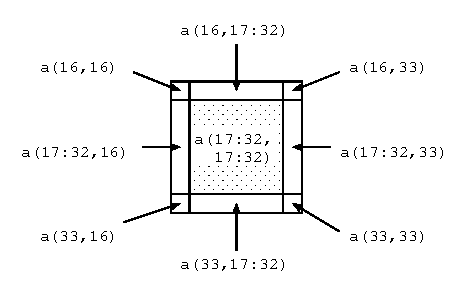
\includegraphics[width=\hsize]{figs/fig3.1.eps}
\end{center}
\caption{Example showing shadow of a two-dimensional array.}
\label{fig3.1}
\end{figure}
\end{minipage}

\vspace{0.5cm}

The node {\tt p(2,2)} has {\tt a(17:32,17:32)} as a data object, and
{\tt a(16,16)}, {\tt a(17:32,16)}, {\tt a(33,16)}, {\tt a(16,17:32)},
{\tt a(33,17:32)}, {\tt a(16,33)}, {\tt a(17:32,33)}, and {\tt a(33,33)}
as shadow objects (Figure \ref{fig3.1}). Among them, {\tt a(16,16)},
{\tt a(33,16)}, {\tt a(16,33)}, and {\tt a(33,33)} are
``obliquely-neighboring'' elements of {\tt p(2,2)}.


\subsection{{\tt template\_fix} Construct}
\label{subsec:template_fix directive}

\subsubsection*{Synopsis}

This construct fixes the shape and/or the distribution of an undefined
template.

\subsubsection*{Syntax}
\Syntax{template\_fix}

\begin{tabular}{ll}
\verb![F]! & \verb|!$xmp| {\tt template\_fix} {\bsquare} \\
 & {\bsquare} {\openb}\verb|(| {\it dist-format} {\openb}, {\it dist-format}{\closeb}... \verb|)|{\closeb} 
   {\it template-name} {\openb}\verb|(|{\it template-spec} {\openb}, {\it template-spec}{\closeb}... \verb|)|{\closeb} \\
 & \\
\verb![C]! & \verb|#pragma xmp|  {\tt template\_fix} {\bsquare} \\
 & {\bsquare} {\openb}\verb|(| {\it dist-format} {\openb}, {\it dist-format}{\closeb}...\verb|)|{\closeb} 
   {\it template-name} {\openb}\verb|(|{\it template-spec} {\openb}, {\it template-spec}{\closeb}... \verb|)|{\closeb} \\
 & \hspace{4cm} or \\
 & {\bsquare} {\openb}\verb|[| {\it dist-format} {\openb}, {\it dist-format}{\closeb}...\verb|]|{\closeb}
   {\it template-name} \verb|[| {\it template-spec} \verb|]|
   {\openb} \verb|[|{\it template-spec} \verb|]|... {\closeb} \\
\end{tabular}
\vspace{0.3cm}

where {\it template-spec} is:

\vspace{0.3cm}

\begin{tabular}{ll}
 \hspace{0.5cm} & {\openb}{\it int-expr} :{\closeb} {\it int-expr} \\
\end{tabular}
\vspace{0.3cm}

and {\it dist-format} is one of:

\vspace{0.3cm}

\begin{tabular}{ll}
 \hspace{0.5cm} & {\tt *} \\
 & {\tt block} {\openb}\verb|(| {\it int-expr} \verb|)|{\closeb} \\
 & {\tt cyclic} {\openb}\verb|(| {\it int-expr} \verb|)|{\closeb} \\
 & {\tt gblock} \verb|(| {\it int-array} \verb|)| \\
\end{tabular}

\subsubsection*{Description}

The {\tt template\_fix} construct fixes the shape and/or the
distribution of the template that is initially undefined, by specifying
the sizes and/or the distribution format of 
each dimension at runtime. Arrays that are aligned with an initially undefined
template must be allocatable arrays, in {\XMPF}, or a pointer (see
Section \ref{sec:Dynamic Allocation of Global Data in C}), in
{\XMPC}, which cannot be allocated until the template is fixed by the
{\tt template\_fix} construct. No constructs that have such a
template in their {\tt on} clause should be encountered until the
template is fixed by the {\tt template\_fix} construct. Any undefined
template can be fixed only once by the {\tt template\_fix} construct in
its scoping unit.

The meaning of the sequence of {\it dist-formats} is the same
as that in the {\tt distribute} directive.

\subsubsection*{Restrictions}

\begin{itemize}
% \item \verb![C]! {\it template-name} must be declared by a {\tt
%       template} directive that lexically precedes the directive.
% \item \verb![C]! {\it nodes-name} must be declared by a {\tt nodes}
%       directive that lexically precedes the directive.
\item When a node encounters a {\tt template\_fix} construct at runtime,
      the template specified by {\it template-name} must be undefined.
\item If the sequence of {\it dist-formats} exists in a {\tt
      template\_fix} construct, it must be identical to the 
      sequence of {\it dist-formats} in the {\tt distribute} directive
      for the template specified by {\it template-name}, except for {\it
      int-array} specified in the parenthesis immediately after {\tt
      gblock}.
\item Either the sequence of {\it dist-formats} or the sequence of {\it
      template-spec}'s should be given.
%\item The {\tt template\_fix} construct must appear in executable
%      context.
\end{itemize}

\subsubsection*{Example}
\Example{template\_fix}

\vspace{0.5cm}
\begin{minipage}{0.46\hsize}
\begin{center}
\begin{XFexample}
!$xmp nodes p(*)
!$xmp template t(:)
!$xmp distribute t(gblock(*)) onto p
real, allocatable :: a(:)
!$xmp align a(i) with t(i)
...
N = ...
M(...) = ...
...
!$xmp template_fix(gblock(M)) t(N)
...
allocate (a(N))
\end{XFexample}
\end{center}
\end{minipage}
%
\begin{minipage}{0.54\hsize}
\begin{center}
\begin{XCexampleR}
#pragma xmp nodes p[*]
#pragma xmp template t[:]
#pragma xmp distribute t[gblock(*)] onto p
double *a;
#pragma xmp align a[i] with t[i]
...
N = ...;
M[] = {...};
...
#pragma xmp template_fix[gblock(M)] t[N]
...
a = xmp_malloc(xmp_desc_of(a), N);
\end{XCexampleR}
\end{center}
\end{minipage}

Because the shape is {\tt t(:)} or {\tt t[:]} and the distribution format is {\tt gblock(*)}, 
the template {\tt t} is initially undefined. The allocatable array
{\tt a} is aligned with {\tt t}. After the size {\tt N} and the
mapping array {\tt M} is defined, {\tt t} is fixed by the {\tt
  template\_fix} construct and {\tt a} is allocated.


In {\XMPC}, it is possible to allocate global arrays at runtime only
when they are one-dimensional.
%
Such an allocation is done by perfoming the following steps.
%
\begin{enumerate}
 \item Declare a pointer to an object of the type of the global array to
       be allocated.
 \item Align the pointer with a template as if it were a one-dimensional
       array.
 \item Allocate a storage of the global size with the function {\tt xmp\_malloc()}
       and assign the result value to the pointer on each node.
\end{enumerate}
%
The functions {\tt xmp\_desc\_of()} and {\tt xmp\_malloc()} are described in section 
\ref{sec:Descriptor of Global Data in C} and \ref{subsec: xmp_malloc}, respectively.

